
\newcommand{\lib}[1]{{\mbox{\normalfont\textsf{#1}}}}
\newcommand{\Rfunction}[1]{{\mbox{\normalfont\texttt{#1}}}}
\newcommand{\Robject}[1]{{\mbox{\normalfont\texttt{#1}}}}
\newcommand{\Rpackage}[1]{{\mbox{\normalfont\textsf{#1}}}}
\newcommand{\Rclass}[1]{{\mbox{\normalfont\textit{#1}}}}

\title{Image analysis for microscopy screens}
\subtitle{Image analysis and processing with \Rpackage{EBImage}}
\author{by Oleg Sklyar and Wolfgang Huber}

\maketitle

The package \Rpackage{EBImage} provides functionality to perform {\em image processing} and {\em image analysis} on large sets of images in a programmatic fashion using the \R{} language.

We use the term {\em image analysis} to describe the extraction of numeric features ({\em image descriptors}) from images and image collections. Image descriptors can then be used for statistical analysis, such as classification, clustering and hypothesis testing, using the resources of \R{} and its contributed packages.

Image analysis is not an easy task, and the definition of image descriptors depends on the problem. Analysis algorithms need to be adapted correspondingly. We find it desirable to develop and optimize such algorithms in conjunction with the subsequent statistical analysis, rather than as separate tasks. This is one of our motivations for writing the \R{}-package \Rpackage{EBImage}.

We use the term {\em image processing} for operations that turn images into images, with the goals of enhancing, manipulating, sharpening, denoising or similar~\citep{R:Russ:2002}. While some image processing is often needed as a preliminary step for image analysis, image processing is not the primary aim of the package. We focus on methods that do not require interactive user input, such as selecting image regions with a pointer etc. Whereas interactive methods can be extremely effective for small sets of images, they tend to have limited throughput and reproducibility.

\Rpackage{EBImage} uses \Rclass{Magick++} interface to the \lib{\cite{R:ImageMagick:2006}} image processing library to implement much of its functionality in image processing and input/output operations.

%--------------------------------------------------
\section*{Cell-based assays}
%--------------------------------------------------

Advances in automated microscopy have made it possible to conduct large scale cell-based assays with image-type phenotypic readouts. In such an assay, cells are grown in the wells of a microtitre plate (often a 96- or 384-well format is used) under a condition or stimulus of interest. Each well is treated with one of the reagents from the screening library and the cells' response is monitored, for which in many cases certain proteins of interest are antibody-stained or labeled with a GFP-tag~\citep{CarpenterSabatini2004, Wiemann2004, MoffatSabatini2006, R:Neumann:2006}.

The resulting imaging data can be in the form of two-dimensional (2D) still images, three-dimensional (3D) image stacks or image-based time courses. Such assays can be used to screen compound libraries for the effect of potential drugs on the cellular system of interest. Similarly, RNA interference (RNAi) libraries can be used to screen a set of genes (in many cases the whole genome) for the effect of their loss of function in a certain biological process~\citep{R:Boutros:2004}.

%--------------------------------------------------
\section*{Importing and handling images}
%--------------------------------------------------

Images in \Rpackage{EBImage} are stored in objects of class \Rclass{Image} that extends the \R{}-class \Rclass{array}. The colour mode is defined by the slot \code{rgb} in \Rclass{Image}; the default mode is {\em grayscale}.

New images can be created with the standard \R{}-constructor \Rfunction{new}, or using the wrapper function \Rfunction{Image}. The following example code generates a \normalfont\textsf{100x100} pixel grayscale image with black and white vertical stripes \footnote{All examples in this article are based on the \lib{BioC 1.9-devel} version of \Rpackage{EBImage}, version 1.3.100 or later}:

\begin{verbatim}
> im <- Image(0.0, c(100,100))
> im[c(1:20, 40:60, 80:100),,] = 1
\end{verbatim}

As mentioned above, \Rpackage{EBImage} interfaces \Rclass{Magick++} for input/output operations. \lib{ImageMagick}, and thus \Rpackage{EBImage}, supports reading and writing of more than 95 image formats including JPEG, TIFF and PNG. The package can read and write multi-page images (image stacks, 3D images) or process multiple files simultaneously. For example, the following code demonstrates how to read all PNG files in the working directory into a single object of class \code{Image}, convert them to grayscale and save the output as a single multi-page TIFF file:

\begin{verbatim}
> files <- dir(pattern=".png")
> im <- read.image(files, rgb=TRUE)
> img <- toGray(im)
> write.image(img, "single_multipage.tif")
\end{verbatim}

Besides operations on local image files, anonymous HTTP and FTP protocols are supported. The package can read from both and it can write to FTP only. These protocols are supported internally by \lib{ImageMagick} and do not use \R{}-connections.

The storage mode of grayscale images is \Rclass{double} (or \Rclass{numeric}), and all \R{}-functions that work with arrays can be directly applied to grayscale images. This includes the arithmetic functions, subsetting, histograms, Fourier transformation, (local) regression etc. For example, the sharpened image in Figure~\ref{figure:sharpening}{\bf c} can be obtained by {\em subtracting} the slightly blurred, scaled in colour version of the original image (Figure~\ref{figure:sharpening}{\bf b}) from its source in Figure~\ref{figure:sharpening}{\bf a}. All pixels that become negative after subtraction are then re-set to background. The source image is a {\em subset} of the original microscopic image. Hereafter, variables in the code are given the same literal names as the corresponding image labels (e.g. data of variable \code{a} are shown in Figure ~\ref{figure:sharpening}~{\bf a}, \code{b} -- in {\bf b}, and \code{C} -- in {\bf c}, etc).

\begin{verbatim}
> orig <- read.image("ch2.png")
> a <- orig[150:550, 120:520,]
> b <- blur(0.5 * a, 80, 5)
> C <- a - b
> C[C < 0] = 0
> C <- normalize(C)
\end{verbatim}

One can think of this code as of a naive, but fast and effective, version of the {\em unsharp mask} filter; a more sophisticated implementation from the \lib{ImageMagick} library is provided by the function \Rfunction{unsharpMask} in the package.

\begin{figure}
\vspace*{.1in}
\begin{center}
\scalebox{1.1}{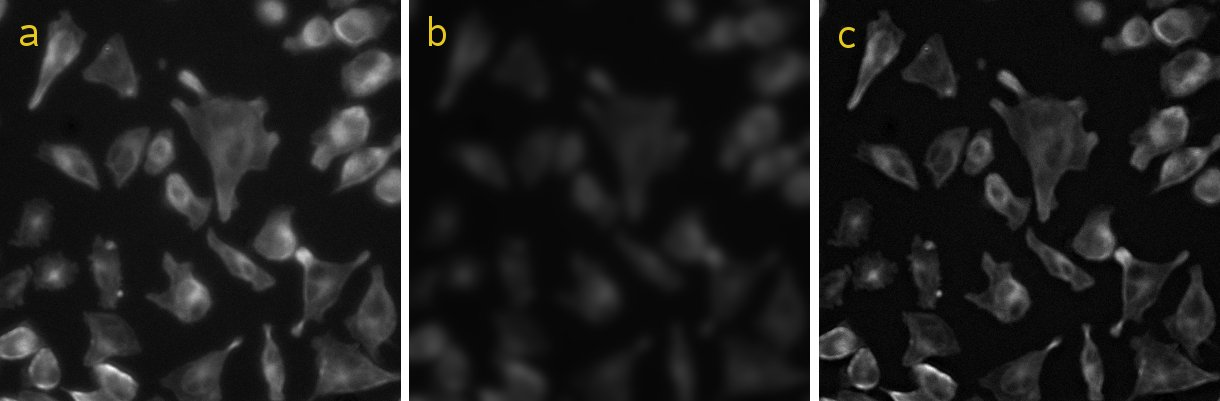
\includegraphics{sharpen.jpg}}
\end{center}
\caption{\label{figure:sharpening}
    Implementation of a simple {\em unsharp mask} filter: (a) source image, (b) blurred colour-scaled image, (c) sharpened image after normalization}
\end{figure}

Some of the image analysis routines in \Rpackage{EBImage} assume grayscale data in the interval $[0,1]$, but formally there are no restrictions on the range.

The storage mode of RGB-images is \Rclass{integer}, and we use the three lowest bytes to store red (R), green (G) and blue (B) values each in the integer-based range of $[0, 255]$. Because of this, arithmetic and other functions are generally meaningless for RGB-images; although they can be useful in some special cases, as shown in the example code in the following section. Support for RGB-images in \Rpackage{EBImage} is included to enhance the display of the analysis results. Most analysis routines require grayscale data though.

%--------------------------------------------------
\section*{Image processing}
%--------------------------------------------------

The \lib{ImageMagick} library provides a number of image processing routines, so-called {\em filters}. Many of those are ported to \R{} by the package. The missing ones will be added at a later stage. We have also implemented additional image processing routines that we found useful for our work on cell-based assays.

Filters are implemented as functions acting on objects of class \Rclass{Image} and returning a new \Rclass{Image}-object of the same or appropriately modified size. One can divide them into four categories: image {\em enhancement}, {\em segmentation}, {\em transformation} and {\em colour correction}. Some examples are listed below. 

\begin{description}
    \setlength{\itemsep}{0in}
    \item[sharpen, unsharpMask] generate sharpened versions of the original image. 
    \item[gaussFilter] applies the Gaussian blur operator to the image, softening sharp edges and noise.
    \item[thresh] segments a grayscale image into a binary black-and-white image by the adaptive threshold algorithm.
    \item[mOpen, mClose] use erosion and dilation to enhance edges of objects in binary images and to reduce noise.
    \item[distMap] performs a Euclidean distance transform of a binary image, also known as {\em distance map}. On a distance map, values of pixels indicate how far are they away from the nearest background. Our implementation is adapted from the~\lib{\cite{R:SIP:2005}} and is based on the algorithm by~\cite{R:Lotufo+Zampirolli:2001}.
    \item[normalize] shifts and scales colours of grayscale images to a specified range, normally $[0,1]$.
    \item[sample.image] proportionally resizes images.
\end{description}

The following code demonstrates how grayscale images recorded using three different microscope filters (Figure~\ref{figure:channels}~{\bf a}, {\bf b} and {\bf c}) can be put together into a single {\em false-colour} representation (Figure~\ref{figure:channels}~{\bf d}), and conversely, how a single false-colour image can be decomposed into its individual channels.

\begin{figure}
\vspace*{.1in}
\begin{center}
\scalebox{1.1}{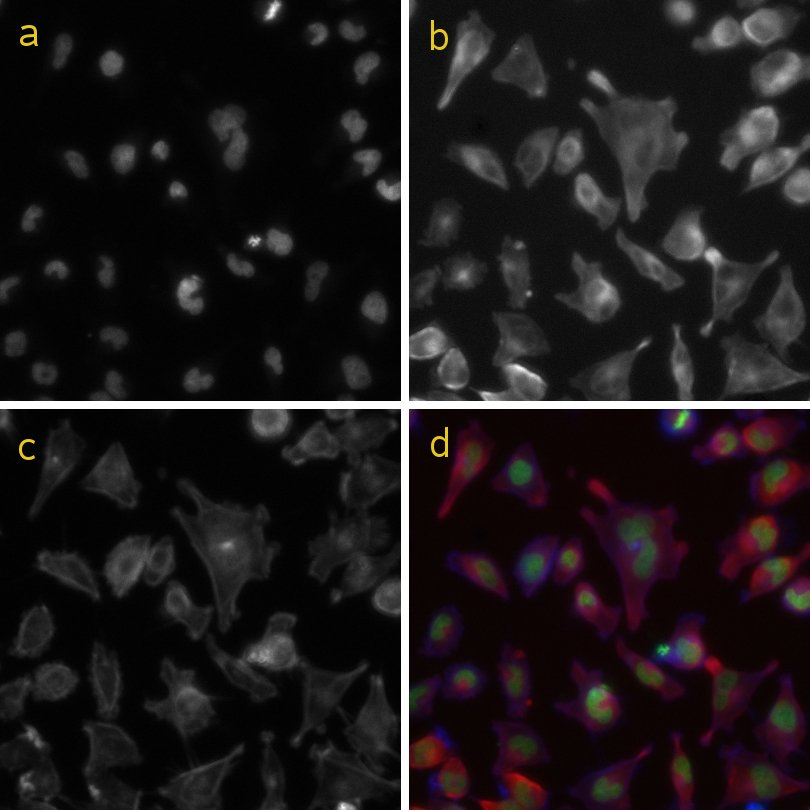
\includegraphics{channels.jpg}}
\end{center}
\caption{\label{figure:channels}
    Composition of a false-colour image (d) from a set of grayscale microscopy images for three different luminescent compounds: (a) -- DAPI, (b) -- tubulin and (c) -- phalloidin
}
\end{figure}

\begin{verbatim}
> files <- c("ch1.png","ch2.png","ch3.png")
> orig <- read.image(files, rgb=FALSE)
> abc <- orig[150:550, 120:520,]
> a <- toGreen(abc[,,1])         # RGB
> b <- toRed(abc[,,2])           # RGB
> d <- a + b + toBlue(abc[,,3])
> C <- getBlue(d)                # gray
\end{verbatim}

%--------------------------------------------------
\section*{Displaying images}
%--------------------------------------------------

Images can be displayed in two different ways. \Rpackage{EBImage} defines method \Rfunction{display} that shows images in an interactive X11 window, where image stacks can be animated and browsed through. This function is fast, but (so far) it fails on some systems, including all tested \lib{MacOS X} and some \code{ssh -X} sessions. It does not use graphic devices of \R{}, and thus cannot be redirected to any of those. As a workaround for grayscale images \Rpackage{EBImage} provides method \Rfunction{plot.image}, which is a wrapper around the standard function \Rfunction{image} from the \Rpackage{graphics} package. Since each pixel is drawn as a polygon, \Rfunction{plot.image} is slow. Additionally it can plot only the first image of a 3D stack. A code example is shown below.

\begin{verbatim}
> display(abc)         # displays all 3
> plot.image(abc[,,2]) # can display just 1
\end{verbatim}

%--------------------------------------------------
\section*{Drawables}
%--------------------------------------------------

Pixel values can be set either by using the convential subset assignment syntax for arrays (as in the third code example, \code{C[C < 0] = 0}) or by using {\em drawables}. \Rpackage{EBImage} defines the following instantiable classes for drawables (derived from the virtual \code{Drawable}): \code{DrawableCircle}, \code{DrawableLine}, \code{DrawableRect} and \code{DrawableEllipse}. The stroke and fill colours, the fill opacity and the stroke width can be set in the corresponding slots of \Rclass{Drawable}. As the opportunity arises, we plan to provide drawables for text, poly-lines and polygons. Drawables can be drawn on \Rclass{Image}s with the method \code{draw}; both grayscale and RGB images are supported with all colours automatically converted to gray levels on grayscale images.

The code below illustrates how drawables can be used to mark the positions and relative sizes of the nuclei detected from the image in Figure~\ref{figure:channels}{\bf a}. It assumes that \Robject{x1} is the result of the \Rpackage{EBImage} function \Rfunction{wsObjects}, which uses a watershed-based image segmentation for object detection. \Robject{x1} contains matrix \Robject{objects} with object coordinates (columns 1 and 2) and areas (column 3). The resulting image is shown in Figure~\ref{figure:drawables}{\bf b}. This is just an illustration, i.~e. we do not assume circular shapes of nuclei. For comparison, originally detected nuclei are colour-marked in Figure~\ref{figure:drawables}{\bf a} using the \Rpackage{EBImage} function \Rfunction{wsPaint}:
%
\begin{verbatim}
> src <- toRGB(abc[,,1])
> x <- x1$objects[,1]
> y <- x1$objects[,2]
> r <- sqrt(x1$objects[,3] / pi)
> cx <- DrawableCircle(x, y, r)
> cx@strokeColor <- "yellow"
> cx@doFill <- FALSE
> b <- draw(src, cx)
> a <- wsPaint(x1, src)
\end{verbatim} 
%$

%FIXME - can we use this syntax instead?
%cx <- DrawableCircle(x, y, r, strokeColor="#66BB00",
%  doFill=TRUE, fillOpacity=0.4, fillColor <- "#559900")

\begin{figure}
\vspace*{.1in}
\begin{center}
\scalebox{1.1}{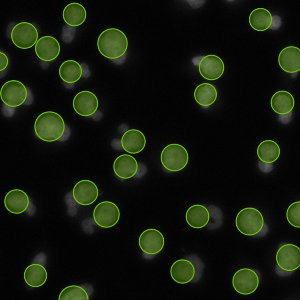
\includegraphics{drawables.jpg}}
\end{center}
\caption{\label{figure:drawables}
    Colour-marked nuclei detected with function \Rfunction{wsObjects}: (a) -- as detected, (b) -- illustrated by \Rclass{DrawableCircle}'s.
}
\end{figure}

%------------------------------------------------------------
\section*{Analysing an RNAi screen}
%------------------------------------------------------------

Consider an experiment in which images like in Figure~\ref{figure:channels} were recorded for each of $\approx$ 20,000 genes, using a whole-genome RNAi library to test the effect of gene knock-down on cell viability and appearance. Among the image descriptors of interest are the number, position, size, shape and the fluorescent intensities of cells and nuclei. 

\Rpackage{EBImage} provides functionality to identify objects in images and to extract image descriptors listed above in the function \Rfunction{wsObjects}. The function identifies different objects in parallel using a modified watershed-based segmentation algorithm and using image distance maps as input. The result is a list of three matrix elements \Robject{objects}, \Robject{pixels} (indices of pixels constituting the objects) and \Robject{borders} (indices of pixels constituting the object boundaries). If the supplied image is an image stack, the result is a list of such lists. The matrix \Robject{objects} has objects in its rows and their features in its columns: the $x$ and $y$ coordinates, size, intensity (if a reference image, \Robject{ref}, is supplied to \Robject{wsObjects}), perimeter and the number of pixels on the image edge. Objects on the edges of images are automatically removed if the ratio of the detected edge pixels to the perimeter is larger than a value specified.

For every gene, the image analysis workflow looks, therefore, as follows: load and normalize images, perform image segmentation, enhance the segmented images by morphological opening and closing, generate distance maps and use them to identify cells and nuclei and to extract image descriptors, and, finally, generate image previews with the identified objects marked. 

Object descriptors can then be analysed statistically to cluster genes by their phenotypic effect, generate a list of genes that should be studied further in more detail (hit list), e.~g. genes that have a specific phenotypic effect of interest, etc. The image previews can be used to verify and audit the performance of the algorithm through visual inspection. 

A schematic implementation is illustrated in the following example code and in the corresponding images in Figure~\ref{figure:analysis} (variable names correspond to image letter notations). Here we omit the step of nuclei detection (object \Robject{x1}), from where the matrix of nuclei coordinates (object \Robject{seeds}) is retrieved to serve as starting points for the cell detection. The nuclei detection is done analogously to the cell detection without specifying starting points.

\begin{figure}
\vspace*{.1in}
\begin{center}
\scalebox{1.1}{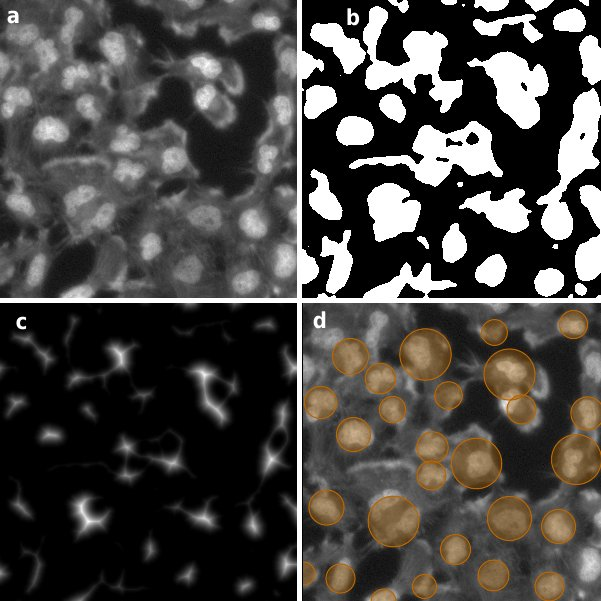
\includegraphics{analysis.jpg}}
\end{center}
\caption{\label{figure:analysis}
Illustration of the object detection algorithm: (a) -- {\em sqrt}-brightened combined image of nuclei (DAPI from Figure~\ref{figure:channels}{\bf a}) and cells (phalloidin from Figure~\ref{figure:channels}{\bf c}); (b) -- image {\bf a} after {\em blur} and {\em adaptive thresholding}; (c) -- image {\bf b} after morphological {\em opening} followed by {\em closing}; (d) -- normalized {\em distance map} generated from image {\bf c}; (e) -- outlines of cells detected using \Rfunction{wsObjects} drawn on top of the RGB image from Figure~\ref{figure:channels}{\bf d}; (f) -- colour-mapped cells and nuclei as detected with \Rfunction{wsObjects} (one unique colour per object)
}
\end{figure}

\begin{verbatim}
> for (X in genes) {
+  files <- dir(pattern=X)
+  orig <- read.image(files)
+  abc <- normalize(orig, independent=TRUE)
+  i1 <- abc[,,1]
+  i2 <- abc[,,2]
+  i3 <- abc[,,3]
+  a <- sqrt(normalize(i1 + i3))
+  b <- thresh(a, 300, 300, 0.0, TRUE)
+  C <-  mOpen(b, 1, mKernel(7))
+  C <- mClose(C, 1, mKernel(7))
+  d <- distMap(C)  # displayed normalized
+  # x1 <- wsObjects(... - nuclei detection
+  seeds <- x1$objects[,1:2]
+  x2 <- wsObjects(d, 30, 10, .2, seeds, i3)
+  rgb <- toGreen(i1)+toRed(i2)+ toBlue(i3)
+  e <- wsPaint(x2, rgb, col="white",fill=F)
+  f <- wsPaint(x2, i3, opac = 0.15)
+  f <- wsPaint(x1, f, opac = 0.15)
+ }
\end{verbatim}
%$

Note that here we adopted the \emph{record-at-a-time} approach: image data, which can be huge, are stored on a mass-storage device and are loaded into RAM in portions of just a few images at a time.

\section*{Summary}

\Rpackage{EBImage} brings image processing and image analysis capabilities to \R. Its focus is the programmatic (non-interactive) analysis of large sets of similar images, such as those that arise in cell-based assays for gene function via RNAi knock-down. Image descriptors extracted as the result of analysis of such images can be analysed further using existing \R{}-functionalities in machine learning (clustering, classification) and hypothesis testing.

Our future developments in image analysis will focus primarily on more accurate object detection and on algorithms for feature/descriptor extraction, and eventually on image registration, alignment and object tracking. Algorithms for the statistical analysis of image descriptors will be developed as part of a separate package that uses \Rpackage{EBImage} for image processing and analysis. In addition, one can imagine many other useful features, for example, support for more \lib{ImageMagick} functions and better display options (e.\,g.\ using GTK). Contributions or collaborations on these or other topics are welcome.

%--------------------------------------------------
\section*{Availability}
%--------------------------------------------------

\Rpackage{EBImage} is available from \lib{BioConductor} (\url{www.bioconductor.org}). The built-in functions \Rfunction{updateEBImage} and \Rfunction{updateEBImageDev} enable updating the package to the lastest stable or the latest development version, correspondingly, between the releases of \lib{BioConductor}.

The package was tested to work on 32 and 64 bit UNIX and Linux systems, and with minor limitations on \lib{MacOS X} (the \Rfunction{plot.image} function should be used instead of \Rfunction{display} on \lib{MacOS X}). \lib{MS Windows} version should be available shortly. \lib{EBImage} depends on \lib{Magick++-devel}, which needs to be present on the system prior to the compilation of the package. Please refer to the \file{INSTALL}-file included with the package for troubleshooting system-specific installation issues.

\section*{Acknowledgements}

We thank F.~Fuchs and M.~Boutros for providing their miscroscopy data and for many stimulating discussions about the technology and the biology, R.~Gottardo and F.~Swidan for testing the package on \lib{MacOS X} and the European Bioinformatics Institute (EBI), Cambridge, UK, for financial support.

\begin{thebibliography}{1}
\expandafter\ifx\csname natexlab\endcsname\relax\def\natexlab#1{#1}\fi
\expandafter\ifx\csname url\endcsname\relax
  \def\url#1{{\tt #1}}\fi

\bibitem[Boutros et al.(2004)]{R:Boutros:2004}
  M.~Boutros, A.~Kiger, S.~Armknecht, \textit{et al.}
  \newblock Genome-wide RNAi analysis of cell growth and viability in Drosophila.
  \newblock {\em Science}, 303:832--835, 2004.

%\bibitem[Fuchs and Boutros(2006)]{R:Fuchs+Boutros:2006}
%    F.~Fuchs and M.~Boutros.
%    \newblock Cellular phenotyping by RNAi.
%    \newblock {\em Brief Funct Genomic Proteomic.}, 5:52--56, 2006.

\bibitem[Carpenter and Sabatini (2004)]{CarpenterSabatini2004}
  A.~E.~Carpenter and D.M.~Sabatini.
  \newblock Systematic genome-wide screens of gene function.
  \newblock {\em Nature Reviews Genetics}, 5:11--22, 2004.

%\bibitem[Carpenter et al.(in preparation)]{R:Carpenter:prep}
%    A.~E.~Carpenter, T.~R.~Jones, M.~Lamprecht, \textit{et al.}
%    \newblock CellProfiler: image analysis for high throughput microscopy.
%    \newblock {\em In preparation}.
%    \newblock URL \url{http://www.cellprofiler.org/}

\bibitem[ImageMagick(2006)]{R:ImageMagick:2006}
    ImageMagick: software to convert, edit, and compose images.
    \newblock {\em Copyright: ImageMagick Studio LLC}, 1999-2006.
    \newblock URL \url{http://www.imagemagick.org/}

%\bibitem[Jones et al.(2005)]{R:Jones:2005}
%    T.~R.~Jones and A.~E.~Carpenter and P.~Golland.
%    \newblock Voronoi-based segmentation of cells on image manifolds.
%    \newblock {\em ICCV Workshop on Computer Vision for Biomedical 
%    Image Applications}, 535--543, 2005 (conference proceedings).

\bibitem[Lotufo and Zampirolli(2001)]{R:Lotufo+Zampirolli:2001}
    R.~Lotufo and F.~Zampirolli.
    \newblock Fast multidimensional parallel Euclidean distance transform based on mathematical morphology.
    \newblock {\em SIBGRAPI-2001/Brazil}, 100--105, 2001.

\bibitem[Moffat and Sabatini (2006)]{MoffatSabatini2006}
  J.~Moffat and D.M.~Sabatini.
  \newblock Building mammalian signalling pathways with RNAi screens.
  \newblock {\em Nature Reviews Mol. Cell Biol.}, 7:177--187, 2006.

\bibitem[Neumann et al.(2006)]{R:Neumann:2006}
    B.~Neumann, M.~Held, U.~Liebel, \textit{et al.}
    \newblock High-throughput RNAi screening by time-lapse imaging of live human cells.
    \newblock {\em Nature Mathods}, 3\penalty0 (5):\penalty0 385--390, 2006.

\bibitem[Russ (2002)]{R:Russ:2002}
    J.~C.~Russ.
   \newblock The image processing handbook -- 4th ed.
   \newblock CRC Press, {\em Boca Raton}. 732 p., 2002

\bibitem[SIP Toolbox(2005)]{R:SIP:2005}
    SIP Toolbox: Scilab image processing toolbox.
    \newblock {\em Sourceforge}, 2005.
    \newblock URL \url{http://siptoolbox.sourceforge.net/}

\bibitem[Wiemann et al. (2004)]{Wiemann2004}
   S.~Wiemann, D.~Arlt, W.~Huber,  \textit{et al.}
   \newblock From ORFeome to biology: a functional genomics pipeline.
   \newblock {\em Genome Res.} 14(10B):2136--2144, 2004.

\end{thebibliography}


\begin{figure}
\vspace*{.1in}
%\begin{center}
\scalebox{0.5}{
\includegraphics{logo.jpg}}
%\end{center}
\end{figure}

\address{Oleg Sklyar and Wolfgang Huber\\
European Bioinformatics Institute\\ 
European Molecular Biology Laboratory\\
Wellcome Trust Genome Campus\\
Hinxton, Cambirdge\\
CB10 1SD\\
United Kingdom}

\noindent{\email{osklyar@ebi.ac.uk}; \email{huber@ebi.ac.uk}}

